% -----------------------------------------------------------------
% 3. Arquitectura del Sistema
% -----------------------------------------------------------------
\section{Arquitectura del Sistema}

\subsection{Arquitectura General}

\textbf{Poneglyph-Reduce} implementa una arquitectura \textbf{Maestro-Trabajadores} (Master-Workers) distribuida, donde cada componente puede ejecutarse en nodos independientes comunicándose a través de Internet. La arquitectura se basa en tres componentes principales:

\begin{figure}[H]
  \centering
  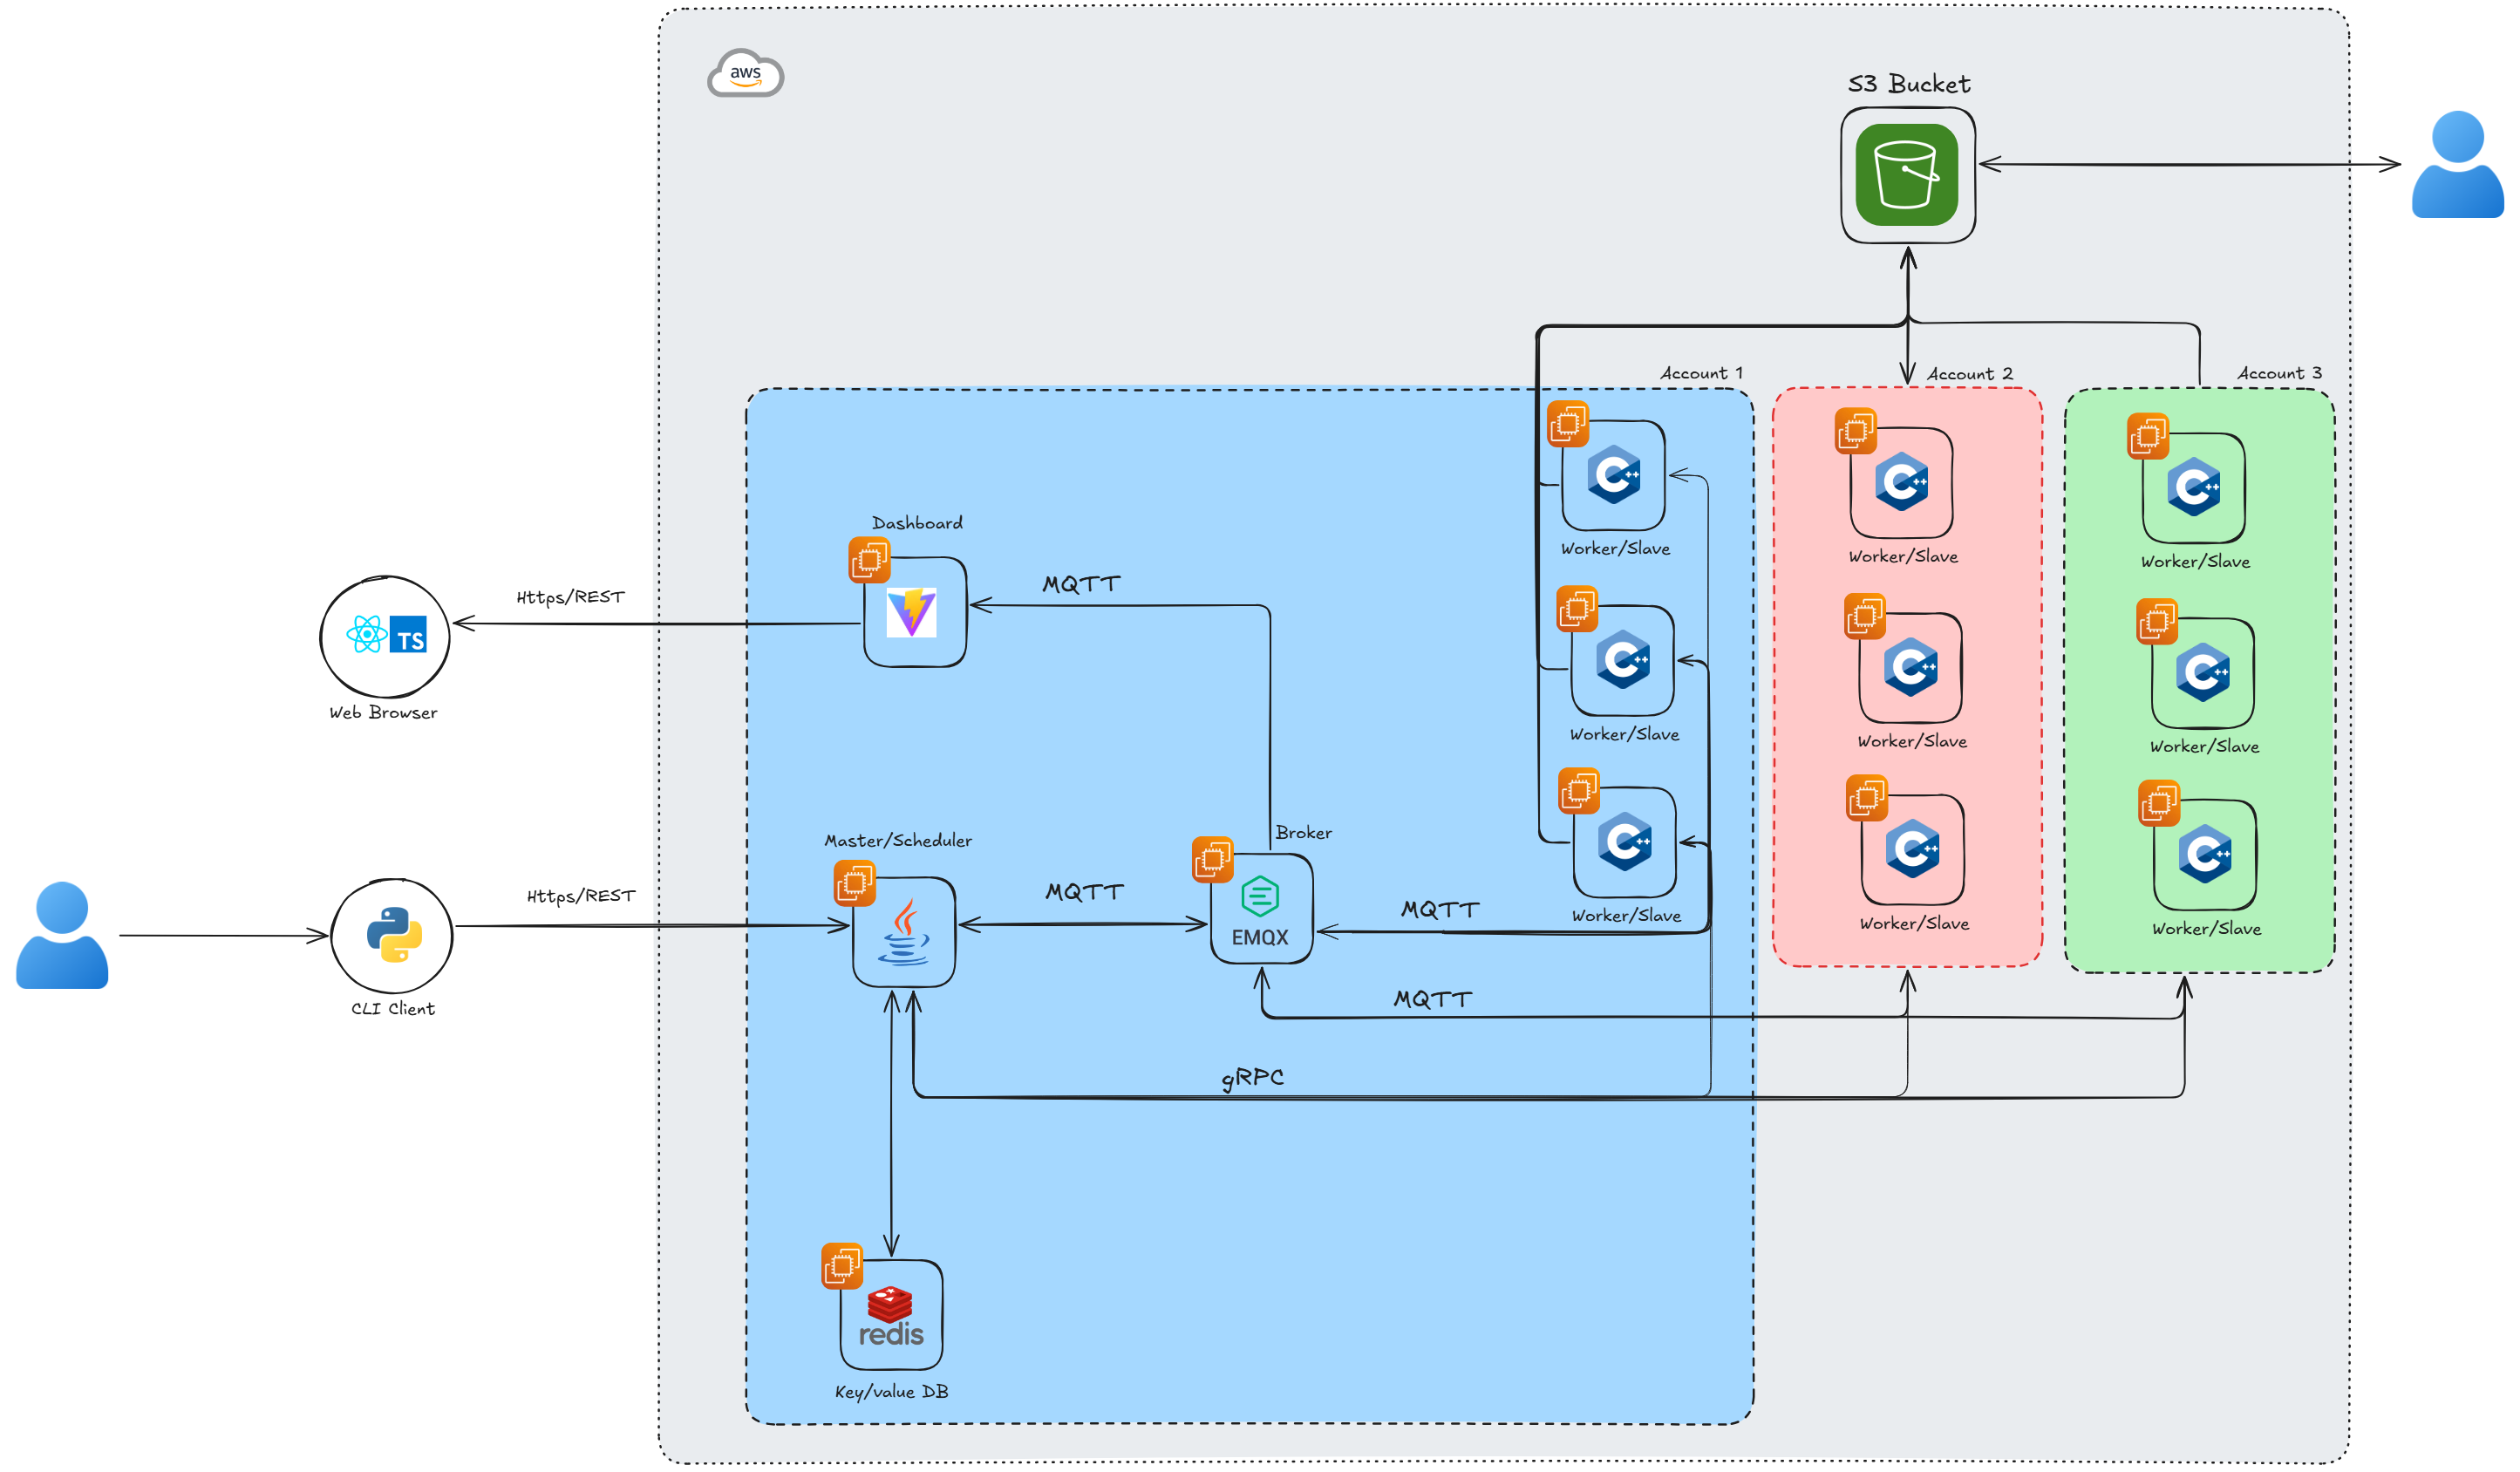
\includegraphics[width=0.9\textwidth]{Figures/0. General/Diagrama Arquitectura.png}
  \caption{Arquitectura general del sistema Poneglyph-Reduce}
  \label{fig:architecture}
\end{figure}

\subsection{Componentes del Sistema}

\subsubsection{Road-Poneglyph (Nodo Maestro)}

El componente maestro, implementado en \textbf{Java 17+}, actúa como coordinador central del sistema y maneja:

\begin{itemize}
    \item \textbf{Recepción de trabajos:} Acepta trabajos del cliente (Python) con scripts map/reduce y configuración
    \item \textbf{Particionamiento:} Divide la entrada en \emph{shards} para distribución
    \item \textbf{Planificación de tareas:} Encola tareas \textbf{MAP} y las asigna a trabajadores disponibles
    \item \textbf{Proceso de mezcla (Shuffle):} Agrupa resultados intermedios por clave y los particiona para reducers
    \item \textbf{Coordinación de reducción:} Emite tareas \textbf{REDUCE} y recolecta resultados
    \item \textbf{Consolidación:} Concatena las salidas de los reducers y expone el resultado final
\end{itemize}

\textbf{Tecnologías utilizadas:}
\begin{itemize}
    \item \textbf{Java 17+ con Gradle:} Plataforma principal de desarrollo
    \item \textbf{HTTP/REST:} API de comunicación con clientes
    \item \textbf{gRPC:} Comunicación eficiente con trabajadores
    \item \textbf{MQTT (EMQX):} Sistema de telemetría y logging en tiempo real
    \item \textbf{Redis:} Persistencia de estado para tolerancia a fallos
\end{itemize}

\subsubsection{Poneglyph (Nodos Trabajadores)}

Los trabajadores, implementados en \textbf{C++20}, son agentes autónomos que:

\begin{itemize}
    \item \textbf{Registro automático:} Se registran con el maestro al inicializar
    \item \textbf{Polling de tareas:} Consultan periódicamente al maestro por trabajo disponible
    \item \textbf{Ejecución de mappers:} Procesan fragmentos de datos asignados ejecutando scripts Python
    \item \textbf{Ejecución de reducers:} Consumen particiones agrupadas y ejecutan reducción
    \item \textbf{Combinación ligera:} Optimizan salidas intermedias antes del envío
    \item \textbf{Heartbeat:} Mantienen comunicación de estado con telemetría MQTT
\end{itemize}

\textbf{Características técnicas:}
\begin{itemize}
    \item \textbf{C++20:} Implementación nativa de alto rendimiento
    \item \textbf{Embedded Python:} Ejecución de scripts map/reduce escritos en Python
    \item \textbf{HTTP Client:} Comunicación con API REST del maestro
    \item \textbf{gRPC Client:} Comunicación binaria eficiente para tareas
    \item \textbf{MQTT Client:} Telemetría y logging en tiempo real
\end{itemize}

\subsubsection{Clover (Cliente)}

El cliente, implementado en \textbf{Python}, proporciona la interfaz para usuarios finales:

\begin{itemize}
    \item \textbf{Envío de trabajos:} Empaqueta scripts map()/reduce(), tamaño de split, número de reducers
    \item \textbf{Seguimiento de estado:} Monitorea el progreso de trabajos en tiempo real
    \item \textbf{Recuperación de resultados:} Obtiene y presenta resultados finales
    \item \textbf{Flexibilidad de interfaz:} Base para CLI, aplicaciones nativas o web
\end{itemize}

\subsection{Infraestructura de Soporte}

\subsubsection{EMQX (MQTT Broker)}

Sistema de mensajería para telemetría y monitoreo en tiempo real:

\begin{itemize}
    \item \textbf{Eventos de trabajos:} Creación, progreso y finalización
    \item \textbf{Heartbeats de trabajadores:} Monitoreo de salud de nodos
    \item \textbf{Logs distribuidos:} Agregación de eventos del sistema
    \item \textbf{Dashboard en tiempo real:} Alimenta la interfaz web de monitoreo
\end{itemize}

\subsubsection{Redis}

Sistema de persistencia clave-valor para tolerancia a fallos:

\begin{itemize}
    \item \textbf{Estado de trabajos:} Especificaciones, contadores y estado actual
    \item \textbf{Registro de trabajadores:} Información de capacidad y disponibilidad
    \item \textbf{Tamaños de particiones:} Metadatos del proceso de shuffle
    \item \textbf{Recuperación de fallos:} Continuación de procesamiento tras interrupciones
\end{itemize}

\subsubsection{Dashboard Web}

Interfaz de monitoreo implementada en \textbf{React + TypeScript}:

\begin{itemize}
    \item \textbf{Visualización en tiempo real:} Estado de trabajos y progreso de tareas
    \item \textbf{Diagrama de flujo:} Representación visual del pipeline MapReduce
    \item \textbf{Logs en vivo:} Stream de eventos MQTT con categorización
    \item \textbf{Métricas del sistema:} Estadísticas de trabajos activos, completados y fallidos
\end{itemize}

\subsection{Modelo de Comunicación}

El sistema implementa un modelo de comunicación híbrido optimizado para diferentes tipos de interacciones:

\subsubsection{Cliente $\leftrightarrow$ Maestro: HTTP/REST}

La comunicación entre cliente y maestro utiliza HTTP/REST por su flexibilidad y universalidad:

\begin{itemize}
    \item \textbf{Flexibilidad de clientes:} Permite fácil migración entre CLI, aplicaciones nativas y web
    \item \textbf{Debugging simplificado:} APIs REST fácilmente inspeccionables
    \item \textbf{Extensibilidad:} Fácil adición de nuevos endpoints
    \item \textbf{Compatibilidad:} Soporte universal en múltiples lenguajes y plataformas
\end{itemize}

\subsubsection{Maestro $\leftrightarrow$ Trabajadores: gRPC}

La comunicación entre maestro y trabajadores utiliza gRPC para máxima eficiencia:

\begin{itemize}
    \item \textbf{Compacidad:} Serialización binaria Protocol Buffers reduce overhead
    \item \textbf{Rendimiento:} Comunicación más rápida para tareas computacionalmente intensivas
    \item \textbf{Tipado fuerte:} Definición clara de contratos de comunicación
    \item \textbf{Eficiencia de red:} Multiplexación HTTP/2 para múltiples streams
\end{itemize}

\subsubsection{Telemetría: MQTT}

Sistema de mensajería asíncrona para eventos y monitoreo:

\begin{itemize}
    \item \textbf{Publicación/Suscripción:} Desacoplamiento entre productores y consumidores
    \item \textbf{Tiempo real:} Eventos inmediatos para dashboard y logging
    \item \textbf{Escalabilidad:} Soporte para múltiples suscriptores sin impacto en rendimiento
    \item \textbf{Persistencia:} Retención de mensajes para análisis posterior
\end{itemize}

\subsection{Tolerancia a Fallos}

El sistema implementa múltiples mecanismos de tolerancia a fallos:

\begin{itemize}
    \item \textbf{Persistencia en Redis:} Estado crítico almacenado para recuperación
    \item \textbf{Heartbeats de trabajadores:} Detección de nodos no disponibles
    \item \textbf{Reintentos de tareas:} Re-encolamiento automático de tareas fallidas
    \item \textbf{Checkpointing:} Guardado incremental de progreso de trabajos
    \item \textbf{Graceful shutdown:} Finalización ordenada de componentes
\end{itemize}
